\documentclass[border=10pt]{standalone}
\usepackage{tikz}
\usetikzlibrary{arrows,positioning,shapes.geometric}
\begin{document}
\



\tikzset{every picture/.style={line width=0.75pt}} %set default line width to 0.75pt        

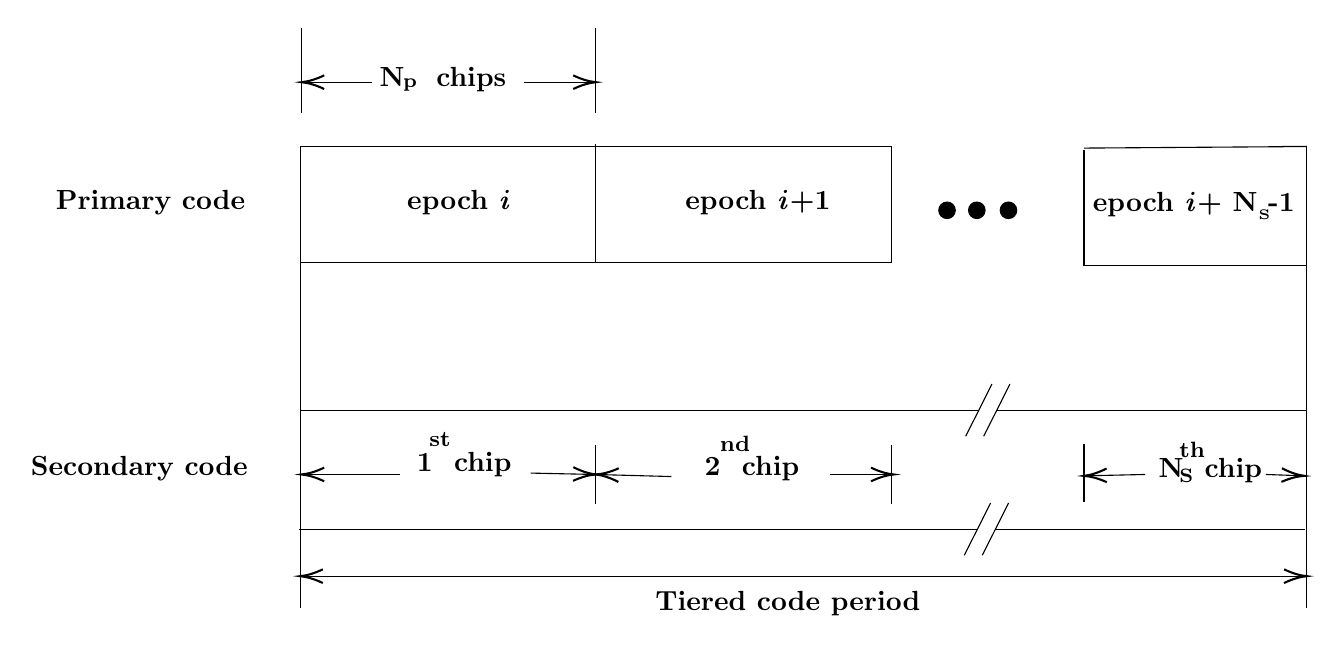
\begin{tikzpicture}[x=0.75pt,y=0.75pt,yscale=-1,xscale=1]
%uncomment if require: \path (0,300); %set diagram left start at 0, and has height of 300

%Straight Lines [id:da15495586894548752] 
\draw    (524,32) -- (524,254.5) ;
%Straight Lines [id:da5506712292647424] 
\draw    (39,32) -- (39,254.5) ;
%Straight Lines [id:da5433715319349757] 
\draw    (39,32) -- (324,32) ;
%Straight Lines [id:da02715971250604632] 
\draw    (416.67,32.75) -- (524,32) -- (512,32) ;
%Straight Lines [id:da40295788607691574] 
\draw    (39,88) -- (324,88) ;
%Straight Lines [id:da6709858164400003] 
\draw    (416.67,89.5) -- (524,89.5) ;
%Straight Lines [id:da12308812297089644] 
\draw    (324,32) -- (324,88) ;
%Straight Lines [id:da775020661044345] 
\draw    (416.67,33.5) -- (416.67,89.5) ;
%Straight Lines [id:da09497172989704072] 
\draw    (181.5,31) -- (181.5,88) ;
%Straight Lines [id:da36038721950652053] 
\draw    (41,239) -- (510,239) -- (522,239) ;
\draw [shift={(524,239)}, rotate = 180] [color={rgb, 255:red, 0; green, 0; blue, 0 }  ][line width=0.75]    (10.93,-3.29) .. controls (6.95,-1.4) and (3.31,-0.3) .. (0,0) .. controls (3.31,0.3) and (6.95,1.4) .. (10.93,3.29)   ;
\draw [shift={(39,239)}, rotate = 0] [color={rgb, 255:red, 0; green, 0; blue, 0 }  ][line width=0.75]    (10.93,-3.29) .. controls (6.95,-1.4) and (3.31,-0.3) .. (0,0) .. controls (3.31,0.3) and (6.95,1.4) .. (10.93,3.29)   ;
%Straight Lines [id:da12157956288884342] 
\draw    (181.5,176) -- (181.5,204) ;
%Straight Lines [id:da6852332210378591] 
\draw    (416.67,175.33) -- (416.67,203.33) ;
%Straight Lines [id:da7747012638794887] 
\draw    (324,176) -- (324,204) ;
%Straight Lines [id:da8492690760045666] 
\draw    (39,159) -- (365.67,159) ;
%Straight Lines [id:da909864699889545] 
\draw    (374.67,159) -- (394.67,159) -- (524,159) ;
%Straight Lines [id:da054605429903387126] 
\draw    (372.33,146.42) -- (359.67,171.58) ;
%Straight Lines [id:da7158011593610226] 
\draw    (381,146.42) -- (368.33,171.58) ;
%Straight Lines [id:da2931213834309231] 
\draw    (38.67,216.33) -- (365.33,216.33) ;
%Straight Lines [id:da8642414917691158] 
\draw    (374,216.33) -- (394,216.33) -- (523.33,216.33) ;
%Straight Lines [id:da9429796644478429] 
\draw    (371.67,203.75) -- (359,228.92) ;
%Straight Lines [id:da9971802380124759] 
\draw    (380.33,203.75) -- (367.67,228.92) ;
%Straight Lines [id:da9596063989994155] 
\draw    (150,189.33) -- (179.5,189.96) ;
\draw [shift={(181.5,190)}, rotate = 181.21] [color={rgb, 255:red, 0; green, 0; blue, 0 }  ][line width=0.75]    (10.93,-3.29) .. controls (6.95,-1.4) and (3.31,-0.3) .. (0,0) .. controls (3.31,0.3) and (6.95,1.4) .. (10.93,3.29)   ;
%Straight Lines [id:da3197669033330087] 
\draw    (294.33,190) -- (323,190) ;
\draw [shift={(325,190)}, rotate = 180] [color={rgb, 255:red, 0; green, 0; blue, 0 }  ][line width=0.75]    (10.93,-3.29) .. controls (6.95,-1.4) and (3.31,-0.3) .. (0,0) .. controls (3.31,0.3) and (6.95,1.4) .. (10.93,3.29)   ;
%Straight Lines [id:da6684976647381153] 
\draw    (504.33,190) -- (520.83,190.59) ;
\draw [shift={(522.83,190.67)}, rotate = 182.06] [color={rgb, 255:red, 0; green, 0; blue, 0 }  ][line width=0.75]    (10.93,-3.29) .. controls (6.95,-1.4) and (3.31,-0.3) .. (0,0) .. controls (3.31,0.3) and (6.95,1.4) .. (10.93,3.29)   ;
%Straight Lines [id:da005153934004900829] 
\draw    (87,190) -- (41.67,190) ;
\draw [shift={(39.67,190)}, rotate = 360] [color={rgb, 255:red, 0; green, 0; blue, 0 }  ][line width=0.75]    (10.93,-3.29) .. controls (6.95,-1.4) and (3.31,-0.3) .. (0,0) .. controls (3.31,0.3) and (6.95,1.4) .. (10.93,3.29)   ;
%Straight Lines [id:da20633389683363146] 
\draw    (217.83,191) -- (183.5,190.06) ;
\draw [shift={(181.5,190)}, rotate = 1.58] [color={rgb, 255:red, 0; green, 0; blue, 0 }  ][line width=0.75]    (10.93,-3.29) .. controls (6.95,-1.4) and (3.31,-0.3) .. (0,0) .. controls (3.31,0.3) and (6.95,1.4) .. (10.93,3.29)   ;
%Straight Lines [id:da92399540634042] 
\draw    (446.17,190) -- (418.67,190.62) ;
\draw [shift={(416.67,190.67)}, rotate = 358.71] [color={rgb, 255:red, 0; green, 0; blue, 0 }  ][line width=0.75]    (10.93,-3.29) .. controls (6.95,-1.4) and (3.31,-0.3) .. (0,0) .. controls (3.31,0.3) and (6.95,1.4) .. (10.93,3.29)   ;
%Straight Lines [id:da43212162953754174] 
\draw    (39.67,-25) -- (39.67,16) ;
%Straight Lines [id:da8347619421235785] 
\draw    (181.5,-25) -- (181.5,16) ;
%Straight Lines [id:da987314582011102] 
\draw    (146.67,1) -- (179.5,1) ;
\draw [shift={(181.5,1)}, rotate = 180] [color={rgb, 255:red, 0; green, 0; blue, 0 }  ][line width=0.75]    (10.93,-3.29) .. controls (6.95,-1.4) and (3.31,-0.3) .. (0,0) .. controls (3.31,0.3) and (6.95,1.4) .. (10.93,3.29)   ;
%Straight Lines [id:da08833944593104714] 
\draw    (41.67,1) -- (73.5,1) ;
\draw [shift={(39.67,1)}, rotate = 0] [color={rgb, 255:red, 0; green, 0; blue, 0 }  ][line width=0.75]    (10.93,-3.29) .. controls (6.95,-1.4) and (3.31,-0.3) .. (0,0) .. controls (3.31,0.3) and (6.95,1.4) .. (10.93,3.29)   ;
%Shape: Circle [id:dp6247864938653165] 
\draw  [fill={rgb, 255:red, 0; green, 0; blue, 0 }  ,fill opacity=1 ] (361.06,62.72) .. controls (361.06,60.53) and (362.83,58.75) .. (365.03,58.75) .. controls (367.22,58.75) and (369,60.53) .. (369,62.72) .. controls (369,64.92) and (367.22,66.69) .. (365.03,66.69) .. controls (362.83,66.69) and (361.06,64.92) .. (361.06,62.72) -- cycle ;
%Shape: Circle [id:dp5722843563375949] 
\draw  [fill={rgb, 255:red, 0; green, 0; blue, 0 }  ,fill opacity=1 ] (346.71,62.72) .. controls (346.71,60.53) and (348.48,58.75) .. (350.68,58.75) .. controls (352.87,58.75) and (354.65,60.53) .. (354.65,62.72) .. controls (354.65,64.92) and (352.87,66.69) .. (350.68,66.69) .. controls (348.48,66.69) and (346.71,64.92) .. (346.71,62.72) -- cycle ;
%Shape: Circle [id:dp05892493621888806] 
\draw  [fill={rgb, 255:red, 0; green, 0; blue, 0 }  ,fill opacity=1 ] (376.31,62.72) .. controls (376.31,60.53) and (378.08,58.75) .. (380.28,58.75) .. controls (382.47,58.75) and (384.25,60.53) .. (384.25,62.72) .. controls (384.25,64.92) and (382.47,66.69) .. (380.28,66.69) .. controls (378.08,66.69) and (376.31,64.92) .. (376.31,62.72) -- cycle ;

% Text Node
\draw (208.9,245) node [anchor=north west][inner sep=0.75pt]   [align=left] {\textbf{Tiered code period}};
% Text Node
\draw (-80,52) node [anchor=north west][inner sep=0.75pt]   [align=left] {\textbf{Primary code}};
% Text Node
\draw (-92,180) node [anchor=north west][inner sep=0.75pt]   [align=left] {\textbf{Secondary code}};
% Text Node
\draw (94,178.17) node [anchor=north west][inner sep=0.75pt]   [align=left] {\textbf{1 \ chip}};
% Text Node
\draw (100,168.33) node [anchor=north west][inner sep=0.75pt]   [align=left] {{\footnotesize \textbf{st}}};
% Text Node
\draw (232.67,180.17) node [anchor=north west][inner sep=0.75pt]   [align=left] {\textbf{2 \ chip}};
% Text Node
\draw (240,170.33) node [anchor=north west][inner sep=0.75pt]   [align=left] {{\footnotesize \textbf{nd}}};
% Text Node
\draw (451.33,180.83) node [anchor=north west][inner sep=0.75pt]   [align=left] {\textbf{N \ chip}};
% Text Node
\draw (461.33,173) node [anchor=north west][inner sep=0.75pt]   [align=left] {{\footnotesize \textbf{th}}};
% Text Node
\draw (461.33,186.33) node [anchor=north west][inner sep=0.75pt]   [align=left] {{\scriptsize \textbf{S}}};
% Text Node
\draw (89.33,52) node [anchor=north west][inner sep=0.75pt]   [align=left] {\textbf{epoch \textit{i}}};
% Text Node
\draw (223.33,52) node [anchor=north west][inner sep=0.75pt]   [align=left] {\textbf{epoch \textit{i}+1}};
% Text Node
\draw (419.67,53) node [anchor=north west][inner sep=0.75pt]   [align=left] {\textbf{epoch \textit{i}+ N\ -1}};
% Text Node
\draw (499.52,61.15) node [anchor=north west][inner sep=0.75pt]   [align=left] {{\tiny \textbf{S}}};
% Text Node
\draw (76,-7.5) node [anchor=north west][inner sep=0.75pt]   [align=left] {\textbf{N \ \ chips}};
% Text Node
\draw (87.33,-2) node [anchor=north west][inner sep=0.75pt]   [align=left] {{\scriptsize \textbf{p}}};


\end{tikzpicture}






   
\end{document}


